\chapter{Global analytics}
This chapter concerns global analytics, used to have an initial view on the real value of the data: goals include understanding what kind of information can be extracted and setting practical fields of interest to make deeper research.

The methodology consists in the application of \textbf{exploratory analysis} and \textbf{descriptive statistics} on the existing dataset.

To have a general idea, the considered approach involves the \textit{whole dataset}: all the available information is included, consisting in the entire time range of 18 years and the totality of patients with related records. Missing or incorrect data is then removed, without imposing additional constraints.

Analysis is performed using:
\begin{itemize}
	\item Diagnoses;
	\item Prescriptions;
	\item Patients' phenotype.
\end{itemize}

Performed operations are simple, such as aggregating, ranking and counting, to avoid high computational costs while obtaining clear and comparable results.

Prescriptions are additionally grouped and measured along with diagnoses, to identify eventual linkage between most popular ones, and focus on discrepancies.

The main purpose of global analytics is highlighting unusual patterns and cross-checking information with external studies, confirming anomalies or restricting the field to existing areas of concern.

\section{Most frequent diseases}
Selection of a subset of diseases is possible after preliminary analysis, of which the most immediate regards frequent appearances in the database. 

There are 9 895 distinct ICD-9 in the \textit{diagnoses} table: of those, the 10 most popular ones in terms of count get selected and shown in table \ref{freqdiagn}.

\begin{table}[h]
	\centering
	\begin{tabular}{c|c|c|c}
		\textbf{\#} & \textbf{ICD-9} & \textbf{Count} & \textbf{Description} \\
		\hline
		1 & 799.9 & 441 131 & Other unspecified cause of morbidity* \\
		\hline
		2 & 401.9 & 305 476 & Unspecified essential hypertension \\
		\hline
		3 & 462 & 301 575 & Acute pharyngitis \\
		\hline
		4 & 521.0 & 274 624 & Dental caries \\
		\hline
		5 & 595.9 & 226 428 & Cystitis, unspecified \\
		\hline
		6 & 464.1 & 221 803 & Acute tracheitis \\
		\hline
		7 & 466.0 & 200 408 & Acute bronchitis \\
		\hline
		8 & 780.7 & 183 721 & Malaise and fatigue \\
		\hline
		9 & 530.81 & 182 897 & Esophageal reflux \\
		\hline
		10 & 724.2 & 176 921 & Lumbago
	\end{tabular}
	\caption{\small Most frequent diseases in 18 years}
	\label{freqdiagn}
\end{table}

The most common ICD-9 (*full name: other unknown or unspecified cause of morbidity and mortality) corresponds to a generic unspecified disease, therefore cannot be subject of detailed analysis.

Other diseases vary through chronic and not, different interested age ranges and different organs of the body: further information can be obtained imposing additional constraints on classification.

\subsection{Most frequent diseases based on age}
Since some diseases are likely to appear within specific ages, patients are grouped into \textbf{ranges} and the most common ICD-9 are counted based on the difference between birthdate and prescription date.

\subsubsection{Age ranges}
The classification method follows \textit{international standards} by United Nations\cite{age}, developed on the basis of existing national practices and recommendations concerning age.

Health classification, in particular, identifies the following ranges to the third level of detail:
\begin{enumerate}
	\item Less than 1 year of age;
	\item 1-14 years of age;
	\item 15-24 years of age;
	\item 25-44 years of age;
	\item 45-64 years of age;
	\item 65+ years of age.
\end{enumerate}

Since the available data concerns general practitioners and not paediatricians, although patients in the younger ages are present there is no warranty of completeness of the doctor-patient relationship, therefore the first two ranges have to be removed.

\subsubsection{Results}
The most common diagnosis for each age range is:
\begin{table}[h]
	\centering
	\begin{tabular}{c|c|c|c}
		\textbf{Range} & ICD-9 & \textbf{Patients} & \textbf{Description} \\
		\hline
		3 & 462 & 49 096 & Acute pharyngitis \\
		\hline
		4 & 799.9 & 119 265 & Other unspecified cause of morbidity \\
		\hline
		5 & 401.9 & 140 510 & Unspecified essential hypertension \\
		\hline
		6 & 401.9 & 123 031 & Unspecified essential hypertension \\
	\end{tabular}
	\caption{\small Most frequent diagnosis for age range}
\end{table}

Since range 4 (25-44) has an unspecified disease as the most common, the 2$^{\text{nd}}$ and 3$^{\text{rd}}$ results are listed:
\begin{enumerate}
	\item 462, 97 040 patients, acute pharyngitis;
	\item 521.0, 83 948 patients, dental caries.
\end{enumerate}
Hypertension is more common among older patients, while young adults are mostly affected by pharyngitis and caries.

Overall, the most popular diagnoses according to age reflect the general rankings.

\subsection{Most frequent diseases based on gender}
Since the database contains more female patients than males, it is expected to have a gap between amounts of diagnoses.

The most frequent diagnoses are however \textbf{unrelated} to gender: there are no relevant differences implying a kind of patients is most likely subject to a disease in the considered subset.

Analytics regarding gender have to be performed choosing a different batch of illnesses, taking the ones which are proven to affect one gender rather than the other.

\subsection{Most common diagnoses based on ICD-9 class}
Making ranks from data on a general level is useful to identify most common diagnoses overall, yet only a limited part of all diseases is taken into account.

Information is sliced only according to aggregated total value, without additional considerations and therefore excluding a wide part of the totality.

Since ICD-9 classification divides diagnoses in \textbf{classes} according to the interested part of the body, extracting the most common illness according to its class allows a better understanding of how important is each group and its \textbf{influence} or relation to the prescriptions. Data can be therefore used to make comparisons.

The whole span of 18 years is used to obtain results, having removed records subject to progressive information loss and incompleteness.

ICD-9 analysis show:
\begin{center}
	\begin{table}[h]
		\makebox[\textwidth][c]{
	\begin{tabular}{c|c|c}
		\textbf{Description} & \textbf{Diagnoses} & \textbf{Count} \\
		\hline
		Infectious and parasitic diseases & Herpes zoster & 28 202 \\
		\hline
		Neoplasms & Benign neoplasm of skin & 41 725 \\
		\hline
		Endocrine and metabolic diseases & Pure hypercholesterolemia & 54 935 \\
		\hline
		Blood and blood-forming organs & Anaemia, unspecified & 71 689 \\
		\hline
		Mental disorders & Dysthymic disturb & 43 303 \\
		\hline
		Nervous system & Acute otitis media & 65 776 \\
		\hline
		Circulatory system & Unspecified essential hypertension & 204 995 \\
		\hline
		Respiratory system & Acute pharyngitis & 212 704 \\
		\hline
		Digestive system & Dental caries & 186 540 \\
		\hline
		Genitourinary system & Cystitis, unspecified & 157 684 \\
		\hline
		Pregnancy and childbirth & Caesarean delivery & 3 144 \\
		\hline
		Diseases of the skin & Dermatitis, unspecified & 93 178 \\
		\hline
		Musculoskeletal system & Lumbago & 116 289 \\
		\hline
		Congenital anomalies & Spondylolisthesis & 883 \\
		\hline
		Conditions in the perinatal period & Subdural and cerebral hemorrhage & 587 \\
		\hline
		Symptoms, signs & Other unspecified cause of morbidity & 262 867 \\
		\hline
		Injury and poisoning & Allergy, unspecified & 74 773 \\
		\hline
		External causes of injury & Pregnant state, incidental & 56 169 \\
	\end{tabular}}
	\caption{\small Most popular diagnoses for ICD-9 class}
\end{table}
\end{center}

Number of prescriptions varies from less than 1 000 to more than 250 000, showing the discrepancy of amount of diagnoses among different classes.

Results reflect general analytics, giving additional insight on other categories having consistent values yet not so high to enter the top rankings, such as dermatitis, anaemia and otitis. 

\section{Chronic illnesses}
A chronic illness is defined as \textit{a disease or condition that usually lasts for 3 months or longer and may get worse over time}\footnote{\href{https://www.cancer.gov/publications/dictionaries/cancer-terms/def/chronic-disease}{Cancer.gov definition}}. They can usually be controlled but not cured.

The major limitation of the database is the lacking of fields representing chronic patients, since illnesses can last any amount of time yet be diagnosed only once, therefore counting and ranking does not give relevant information.

Even identifying a subset of chronic patients based on amount of prescriptions or phenotypes would not result in consistent outcomes, because popular diseases such as hypertension or pharyngitis are spread among all patients and a common reason for periodic visits of the general practitioner.

A patient living with a chronic disease can, in fact, have episodes of sporadic disturbs, therefore there is not a clear distinction between diagnoses and illnesses.

According to researches on chronic diseases in Italy, they tend to occur in older adults, aged 45 or more: the total patients of the dataset falling in this category in 2018 is more than half, 625 309.

Some diffused chronic illnesses are:
\begin{itemize}
	\item Hypertension, with 305 476 diagnoses (almost half of the older adult patients);
	\item Arthritis, with 14 110 diagnoses;
	\item Allergy, with 100 744 diagnoses;
	\item Osteoporosis, with 141 671 diagnoses;
	\item Chronic bronchitis, with 70 537 diagnoses (unrelated to bronchitis);
	\item Asthma, with 121 252 diagnoses;
	\item Crohn's disease, with 859 diagnoses;
	\item Fibromyalgia, with 5 818 diagnoses;
	\item Arrhythmia, with 21 394 diagnoses;
	\item Tumour (all, ICD-9 codes 140-239), 288 659 cases.
\end{itemize}

Although there is a chance that the same disease gets diagnosed more than once to the same patient, values are still high compared to 1 million of patients.

\section{Gender-influenced diseases}
Analytics on most frequent diagnoses according to patient's gender do not show additional relevant information, hence outcomes cannot be obtained using popularity as measure. Prescriptions do not vary either, since their nature is preventive and not curative.

Gender-related diseases might not require a considerable amount of visits of the general practitioner, because either of their chronic aspect or their brief duration.

However, there are important \textit{biological and behavioural differences} between categories. They affect manifestation, epidemiology and pathophysiology of many widespread diseases and the approach to health care. 

Since gender affects a wide range of physiological functions, it has an impact on a wide range of diseases including those of the \textbf{cardiovascular}, pulmonary and autoimmune systems, as well as diseases involving gastroenterology, hepatology, nephrology, endocrinology, haematology and neurology\cite{gender}.

Those differences should reflect on the existing data, showing discrepancies between the number of diagnoses for males and females considering the same disease. To verify the hypothesis, a subset of ICD-9 is selected based on external research, and controls are performed.

It is important to consider that female patients are about 4\% more than males.

\begin{table}[h]
	\centering
	\begin{tabular}{c|c|c}
		\textbf{Description} & \textbf{Diagnoses to males} & \textbf{Diagnoses to females} \\
		\hline
		Cystitis (all) & 59 276 & 173 556 \\
		\hline
		Major depression & 1 141 & 1 483 \\
		\hline
		Anxiety states & 13 926 & 23 455 \\
		\hline
		Substance abuse & 1 054 & 142 \\
		\hline
		Erectile dysfunction & 3 944 & 75 \\
		\hline 
		Osteoporosis & 10 129 & 82 655 \\
		\hline
		Anaemia, unspecified & 20 426 & 51 318 \\
		\hline
		Myocardial infarction & 3 672 & 1 399 \\
	\end{tabular}
	\caption{\small Diseases counts based on gender}
\end{table}

Some categories such as drug abuse include all ICD-9 subsets because of their sparsity, while most common illnesses are counted according to specific typologies to avoid dispersion of information.

It is clear that the selected diseases affect a specific gender than the other: females are likely to get cystitis, anxiety, osteoporosis and anaemia, while males are most subject to substance abuse and erectile dysfunction.

The 75 diagnoses of erectile dysfunction to women are a bright example of wrong diagnosing, and are described as ``decrease of sexual desire'' or even ``frigidity''. Those records have to be excluded from analysis of results, showing information loss cannot always be predicted.

Heart attack is an interesting field to look deeper into: researches show difference of signs between women and men, therefore the bigger number of male diagnoses might be caused by females misinterpreting symptoms. 

Overall, studies related to Campania comply with available information on how diseases affect distinct genders.

\section[Most common prescriptions]{Most common prescriptions based on ATC class}
The purpose of analysing most common prescriptions is to highlight similarities between diseases, and verify whether popular products changed within the past year.

The considered time range is 16 years, divided in spans of 8: 2002-2009 and 2010-2017, to have two comparable pictures of data.

Analytics is performed on the first level of each ATC class, and after extracting each pharmaceutical product, its usage is linked with the most common diagnoses, to understand eventual mutual relationships and connections.

The most common ATC codes for category are counted according to their category (table 6.5).
\begin{center}
	\begin{table}[h]
		\makebox[\textwidth][c]{
	\begin{tabular}{c|c|c|c|c|c}
		\textbf{Class} & \textbf{Description} & \textbf{ATC '02-'09} &\textbf{ N. '02-'09 }& \textbf{ATC '10-'17} & \textbf{N. '10-'17} \\
		\hline
		A & Metabolism & Omeprazole & 717 559 & Pantoprazole & 2 350 368 \\
		\hline
		B & Blood & Acetylsalicylic acid & 1 661 035 & Acetylsalicylic acid & 1 939 484 \\
		\hline
		C & Cardiovascular & Nitroglycerine & 891 586 & Atorvastatine & 1 379 261 \\
		\hline
		D & Epidermis & Calcipotriol & 45 545 & Calcipotriol & 69 505 \\
		\hline
		G & Urinary system & Tamsulosin & 288 840 & Tamsulosin & 494 191 \\
		\hline
		H & Hormones & Levothyroxine & 706 394 & Levothyroxine & 838 499 \\
		\hline
		J & Infections & Amoxicillin & 870 151 & Amoxicillin & 1 522 031 \\
		\hline
		L & Tumours & Tamoxifen & 36 208 & Methotrexate & 62 324 \\
		\hline
		M & Muscular system & Nimesulide & 1 074 632 & Ketoprofen & 740 165 \\
		\hline
		N & Nervous system & Paroxetine & 177 918 & Escitalopram & 348 080 \\
		\hline
		P & Antiparasitic & Hydroxychloroquine & 27 977 & Hydroxychloroquine & 52 150 \\
		\hline
		R & Respiratory & Beclometasone & 412 688 & Beclometasone & 531 337 \\
		\hline
		S & Sensory organs & Timolol & 162 444 & Timolol & 237 196 \\
		\hline
		V & Various & Oxygen & 103 379 & Oxygen & 246 050 \\
	\end{tabular}}
	\caption{\small Most frequent prescription per AIC class}
\end{table}
\end{center}

\subsection{Comparison of results}

\subsubsection{Alimentary tract and metabolism}
The A class shows some potentially concerning results: values of prescriptions of those drugs have tripled from 2002-2009 to 2010-2017. Omeprazole has been substituted by Pantoprazole as top prescribed, yet its prescriptions grew considerably. Both products are for eophageal reflux, which is one of the most diagnoses diseases.

A brief time series analysis on the original \textit{prescriptions} table helps to visualise the growth of the two medicines:
\begin{figure}[h]
	\centering
	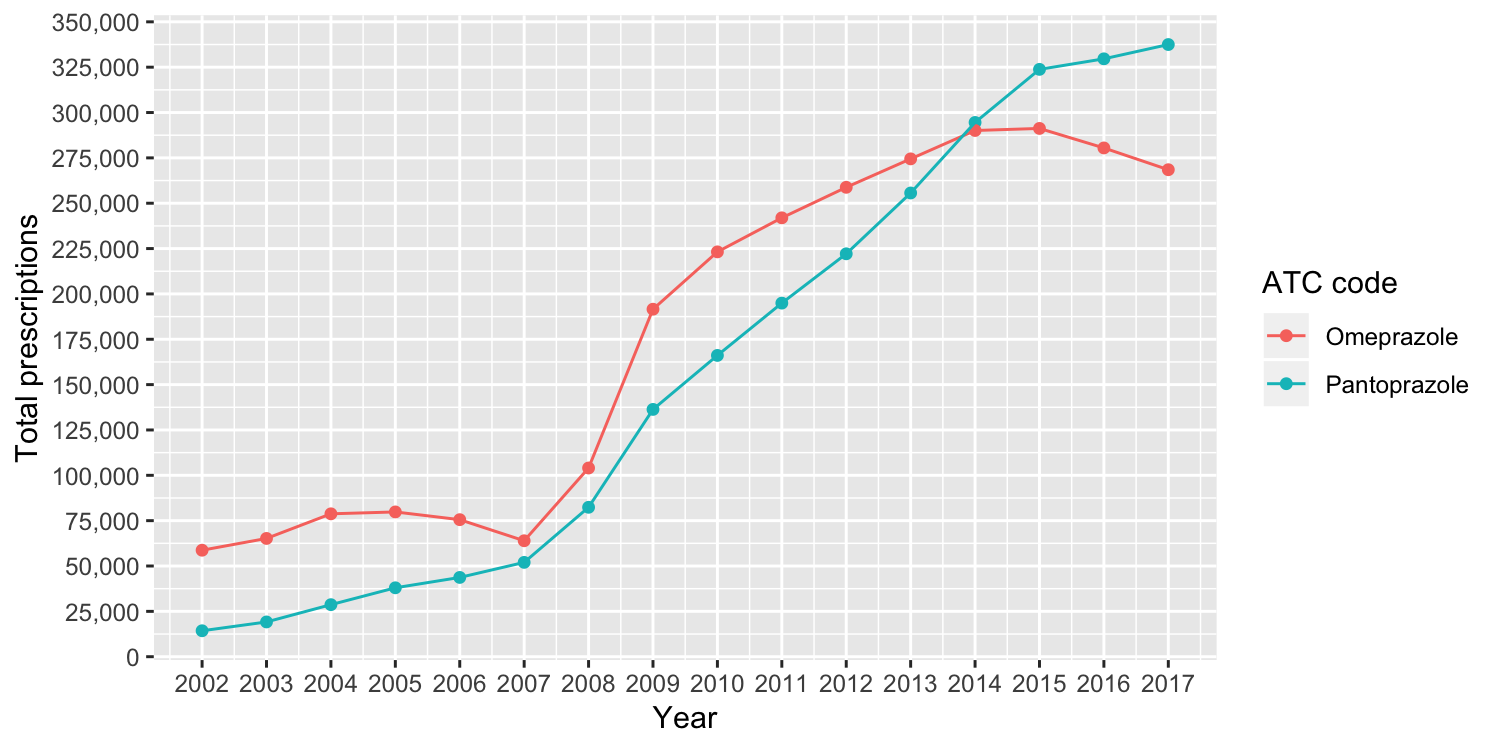
\includegraphics[scale=0.3]{../plots/atc-a-gastro.png}
	\caption{\small Omeprazole and Pantoprazole trends}
\end{figure}

The trend is subject to a drastic change starting from 2007, with a switch of most popular in 2014.

Further examinations confirm that, despite other alimentary tract medicines have lower values, the number of prescriptions of a consistent amount of those is higher than 1 million, yet the raising trend only concerns omeprazole and pantoprazole. 

The hypotheses for changes in patterns are:
\begin{enumerate}
	\item A bigger amount of information falling in the 2010-2017 range;
	\item An effective increase in esophageal reflux and therefore prescriptions related to it.
\end{enumerate}

There are approximatively 18 more millions of tuples overall in 2010-2017, but considering a total amount of 118 millions, the unusual growth cannot be justified by information loss.

Diagnoses of esophageal reflux within years are then counted:
\begin{figure}[h]
	\centering
	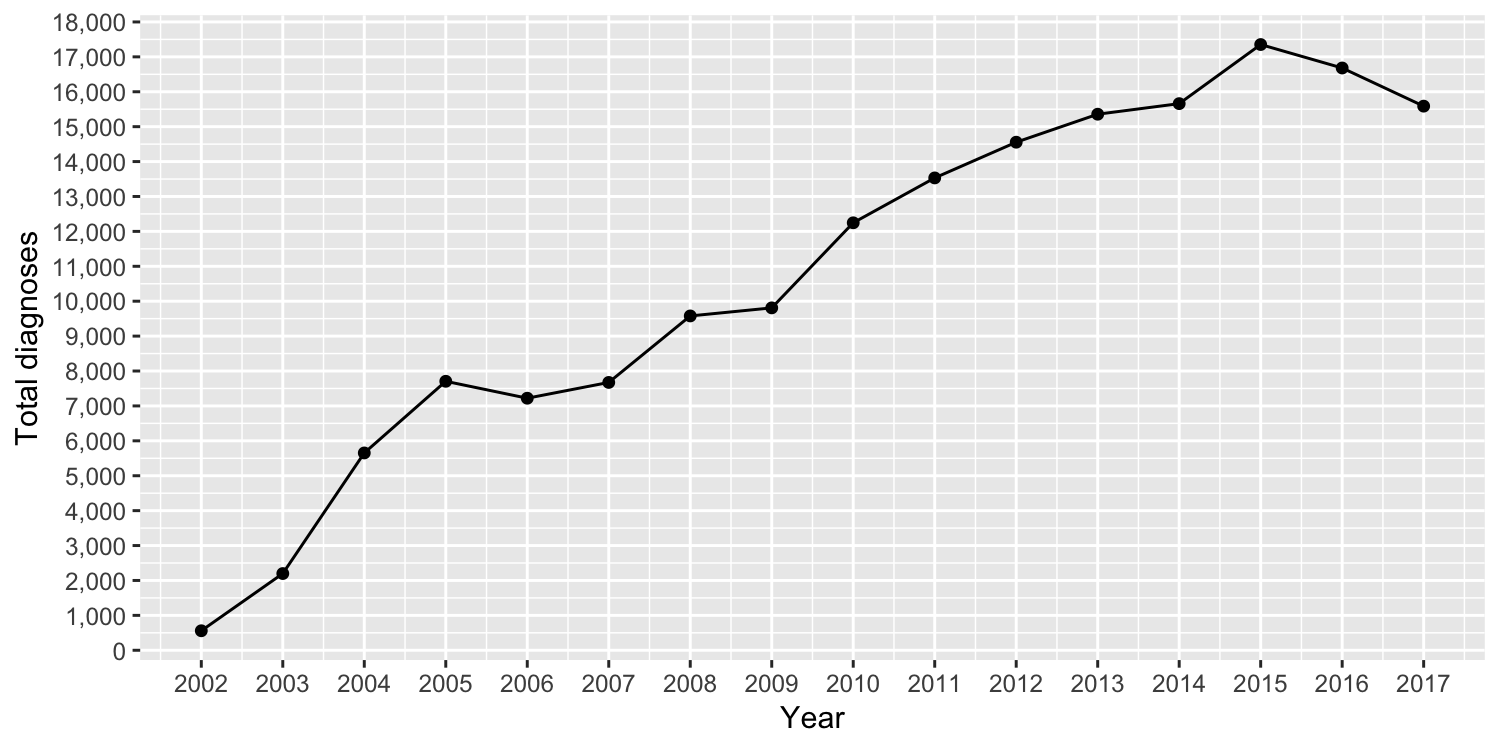
\includegraphics[scale=0.3]{../plots/reflux.png}
	\caption{\small Esophageal reflux trends}
\end{figure}

Values started from less than 1 000 and got to almost 18 000, yet numbers are still too small to explain 300 000 yearly prescriptions. 

Other approaches to have a deeper understanding can involve reconstructing the patients history, or extracting the common diagnoses of patients with a prescription of omeprazole or pantoprazole.

\subsubsection{Blood and blood forming organs}
Blood class has as major product acetylsalicylic acid, which is the active principle of aspirin. This case most likely regards cardio-aspirin, used to prevent and treat heart diseases and as anti-thrombotic.

\subsubsection{Cardiovascular system}
Atorvastatin is the most common medicine in 2010-2017, already confirmed by gender-related analysis. Before 2010, however, the highest-ranked prescriptions was nitroglycerin, followed by amlodipine and simvastatin. 

Numbers suggest a consistent switch of products while dealing with cardiovascular system disease. Values increased, confirming the national issue of heart diseases as principal death cause\cite{ansacuore}.

Those classes of active principle are used for cholesterol control as well, therefore this can have an influence on the prescription trends.

Nitroglycerin lost popularity, probably because of its heavy side effects, unclearness of mechanism or potential danger while interfering with other medicines or defibrillation. 

\subsubsection{Dermatologicals}
Skin medicines aren't subject of relevant mutations: the most popular is still calcipotriol (calcipotriene), a form of vitamin D.

The usage is mainly for psoriasis, which is discordant with the top ranked unspecified dermatitis in the ICD-9 analysis.

There are 30 768 entries in the whole database for ICD-9 codes concerning psoriasis (696.*), approximately $\frac{1}{3}$ respecting to dermatitis and $\frac{1}{4}$ of prescriptions, yet psoriasis is a chronic disease and only gets diagnosed once.

\subsubsection{Genito-urinary system and sex hormones}
Urinary system diseases have as most prescribed drug tamsulosin, for benign prostatic hyperplasia. The most diagnosed issue is cystitis, yet it doesn't usually get treated with a medicine cure.

There are 63 368 cases of prostatic hyperplasia in the whole database, which compared to the $\sim$700 000 total prescriptions doesn't explain such high value. It is not a chronic disease, nor prescribed to women and kids, therefore this phenomenon should be looked further into.

\subsubsection{Systemic hormonal preparations, excluding sex hormones and insulins}
Levothyroxine is one of the most prescribed products in the United States, for hypothyroidism: more than 12\% of the US population is affected by this disease, while in Italy the percentage is around 10\%.

The discrepancy may be due to different lifestyle or lack of diagnoses: in the Campania database there are 29 184 cases in 18 years, which is a small amount compared to the top diagnoses.

\subsubsection{Antiinfectives for systemic use}
Amoxicillin, belonging to the penicillins group, is the most used medicine for infections: its scope covers ear, pharynx, airways, skin, teeth and urinary system infections.

Generally penicillins cover almost the entire amount of prescriptions for infections: this can be related to the high quantity of diagnoses concerning otitis, pharyngitis, laryngitis, bronchitis and tracheitis. 

Number of prescriptions between the two time ranges has doubled, which consists in a starting point to affirm the spread of antibiotic resistance and lack of ethical prescriptions.

\subsubsection{Antineoplastic and immunomodulating agents}
Prescriptions for the antineoplastic category tend to vary: from 2010 there is a prevalence of methotrexate, used to treat tumours, especially leukaemia but also psoriasis, regional enteritis and rheumatoid arthritis.

Previously, the most used product is tamoxifen, for breast cancer. All the other common prescriptions consist in inhibitors, which could mean cases of breast cancer is decreasing.

The database shows 3 805 cases in 2002-2009 and 4 086 in 2010-2017, yet the values are biased because of the bigger amount of information related to the most recent years.

\subsubsection{Musculo-skeletal system}
The popular prescriptions for the muscular system are the same within years, yet their amount drastically changes.

Nimesulide is a nonsteroidal anti-inflammatory drug used for acute pain treatment in orthodontic, rheumatological and gynaecological fields. The medicine has encountered various collateral effects on an European level.

Toxicity and adverse reactions explain the decrease in the number of prescriptions and the switch to Ketoprofene, another nonsteroidal anti-inflammatory drug to treat rheumatological arthritis and osteoarthritis.

\subsubsection{Nervous system}
Powerful antidepressants lead the area of nervous system drugs: although the two products are different in the considered time spans, the class is the same (inhibitors of serotonin receptors).

Prescriptions values are increasing, despite the number of dysthymia diagnoses going from 22 656 to 20 647, therefore other illnesses treated with antidepressant could be spreading (depression, anxiety).

\subsubsection{Antiparasitic products, insecticides and repellents}
Hydroxychloroquine is the only product in this category which is consistently prescribed and passes the 10 000 entries: this is because although it being an antimalarial, it gets used for rheumatological arthritis and lupus.

\subsubsection{Respiratory system}
Different time spans show no relevant differences in the amount of prescriptions of drugs for the respiratory system, yet beclometasone has a detach from all the other medicines (almost double the amount).

\subsubsection{Sensory organs}
Timolol is prescribed for hypertension, one of the most diagnosed diseases overall. There is coherence between diagnoses and prescriptions, yet a difference of approximately 100 000: cases must be increasing.

\subsubsection{Various}
Most common various product is oxygen, having a wide spectrum of uses including cardiac insufficiency, chronic bronchitis and bronchopneumonia: crossing diagnoses happening the same day of this prescription would give an overall idea of the leading diagnoses.

\section{Conclusions}
% fare bene
Overall, data show a general trend of increase of both diagnoses and prescriptions. In most cases, this can be attributed to the presence of more information in the recent years, yet some specific instances raise concerns.

Research could get detailed results through a time series analysis on:
\begin{itemize}
	\item Esophageal reflux and metabolism prescriptions;
	\item Antibiotic resistance;
	\item Tumours and benign hyperplasia. 
\end{itemize}





